\documentclass{article}

\usepackage{polski}
\usepackage{graphicx}
\usepackage{amsmath}
\usepackage{mathtools}
\usepackage{adjustbox}
\usepackage[margin=1in, bmargin=1in, tmargin=0.6in]{geometry}

\author{Paweł Wilkosz}
\title{ON, lista 2 - sprawozdanie}

\begin{document}
\maketitle

\section{Iloczyn wektorowy}

Celem zadania było zastosowanie algorytmów służących do obliczania iloczynu wektorowego zaimplementowanych na poprzedniej liście dla poniższych danych.
$$
x = [2.718281828, -3.141592654, 1.414213562, 0.577215664, 0.301029995]
$$
$$
y = [1486.2497, 878366.9879, -22.37492, 4773714.647, 0.000185049]
$$

Skutkuje to następującymi wynikami.

\begin{center}
  \begin{tabular}{| c | c | c |}
    \hline
    Float32 & \texttt{fronttoback} & -0.2499443 \\
    & \texttt{backtofront} & -0.2043457 \\
    & \texttt{bigtosmall} & -0.25 \\
    & \texttt{smalltobig} & -0.25 \\
    \hline
    Float64 & \texttt{frontoback} &-0.004296342739891585 \\
    & \texttt{backtofront} &-0.004296342739891585 \\
    & \texttt{bigtosmall} &-0.004296342739891585 \\
    & \texttt{smalltobig} &-0.004296342739891585 \\
    \hline
  \end{tabular}
\end{center}

Jak łatwo zauważyć, w arytmetyce Float64 wszystkie algorytmy zwróciły poprawny wynik.

Z powyższego eksperymentu można wnioskować, że algorytmy, jakie zostały użyte do wykonania obliczeń, są poprawne jednak zadanie na poprzedniej liście było źle uwarunkowane.

\section{Wizualizacja funkcji}

Zadanie polegało na wykorzystaniu różnych programów do wizualizacji w celu narysowania wykresu funkcji $f(x) = e^x * \ln (1 + e^{-x})$.
Ponizej widoczne są wyniki tego eksperymentu przy użyciu programów GNU Plot i Wolfram Alpha.

\begin{center}
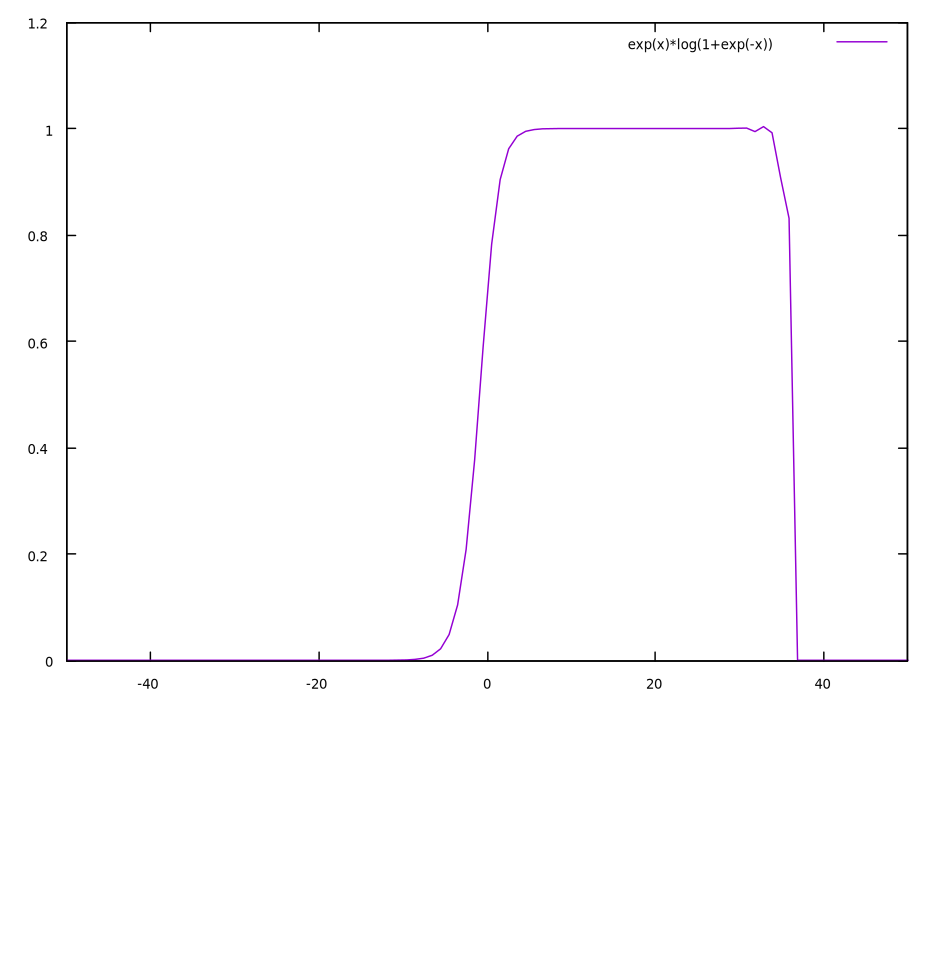
\includegraphics[width=0.45\textwidth]{img/gnuplot.png}
\includegraphics[width=0.45\textwidth]{img/wolfram_plot.png}
\end{center}

Można zaobserwować, że oba programy okazały się niedokładne dla podobnych wartości i pokazują wartości nie mające sensu.

W celu sprawdzenia poprawnosci powyższych wykresów można wykorzystać granicę badanej funkcji.

$$
lim_{n \to \infty} f(x) = 1
$$

Fakt, iż wykresy wygenerowane przy pomocy wspomnianych programów nie zbiegają do wartości $1$, pozwala stwierdzić, że nie są one odporne na błędy obliczeń występujące w działaniu $1+e^{-x}$, które dla dużych $x$ daje wynik $1$.
Jako, że błąd ten wystąpił w dwóch renomowanych programach, można wywnioskować, że jest on trudny, lub niemożliwy, do uniknięcia a problem leży w uwarunkowaniu zadania.

\section{Układ równań liniowych}

Celem zadania było porównanie metod rozwiązywania układów równań liniowych przy pomocy mnożenia macierzy w języku Julia.

Macierze współczynników były generowane na dwa sposoby:
\begin{itemize}
  \item macierz Hilberta stopnia $n : n \in [1,20]$
  \item macierz losowa stopnia $n : n \in \{5,10,20\}$ o stopniu uwarunkowania $c : c\in \{1, 10, 10^3, 10^7, 10^12, 10^16\}$.
\end{itemize}

W każdym przypadku rozważamy układ którego rozwiązaniem jest wektor o wszystkich współrzędnych równych $1$.
Do obliczenia wyniku służyły dwie metody
\begin{itemize}
  \item eliminacja Gaussa - \texttt{A\textbackslash b}
  \item mnożenie przez macierz odwrotną - \texttt{inv(A)*b}
\end{itemize}

Błędy względne dla wygenerowanych macierzy zostały przedstawione w tabelach \ref{hilbertmatrix} (macierz Hilberta) i \ref{randommatrix} (macierz losowa).

Można zaobserwować, że w przypadku elmiinacji Gaussa błędy są niższe niż w przypadku mnożenia przez macierz odwrotną.
Ma to miejsce jednak jedynie dla macierzy Hilberta, w przypadku których błędy są wyższe niż dla macierzy losowych.
W przypadku macierzy losowych różnice w błędach dla obu metod są pomijalne.
Dla obu metod jednak błędy narastają wraz ze wskaźnikiem uwarunkowania macierzy.
Przykład macierzy generowanej losowo pokazuje, że wplyw rzędu macierzy na błędy obliczeń jest pomijalny.

Pozwala to wywnioskować, że metoda eliminacja Gaussa pozwala zmniejszyć błędy obliczeń, jednak dla macierzy o dużym wskaźniku uwarunkowania, nie możemy liczyć na dokładność obliczeń.
Funkcja \texttt{cond} może być pomocna w celu oszacowania potencjalnych niedokładności w wyniku.


\begin{table}[!htpb]
  \centering
  \begin{tabular}{| c | c | c | c | c |}
    \hline
    stopień & wskaźnik uwarunkowania & rząd & błąd \texttt{A\textbackslash b} & błąd \texttt{inv(A)*b} \\
    \hline
    1 & 1.0 & 1 & 0.0 & 0.0\\
    2 & 19.28147006790397 & 2 & 4.227603326225575e-16 & 1.4043333874306803e-15\\
    3 & 524.0567775860644 & 3 & 6.312995352117186e-16 & 0.0\\
    4 & 15513.738738928929 & 4 & 4.1048907912680814e-13 & 6.43463044904617e-13\\
    5 & 476607.25024224253 & 5 & 5.1522140525928354e-12 & 6.508012930390446e-12\\
    6 & 1.495105864125091e7 & 6 & 1.5596145705873347e-10 & 3.188721720715103e-10\\
    7 & 4.7536735637688667e8 & 7 & 1.7795819462095408e-8 & 1.1617642611045831e-8\\
    8 & 1.5257575516147259e10 & 8 & 1.9006770736440594e-7 & 5.001414952694125e-7\\
    9 & 4.9315408927806335e11 & 9 & 1.9032599462688394e-6 & 1.1410119123249102e-5\\
    10 & 1.6024859712306152e13 & 10 & 0.00029008871550622196 & 0.00036330943448230086\\
    11 & 5.2210348947688544e14 & 10 & 0.011424743836176894 & 0.00993429095097543\\
    12 & 1.7255427417341868e16 & 11 & 0.2457035383680344 & 0.29621111105817555\\
    13 & 7.126491965424366e17 & 11 & 40.7486694719936 & 12.72679701952435\\
    14 & 6.101307732044041e17 & 11 & 3.3928217227097677 & 2.3263320263544234\\
    15 & 4.223311222761075e17 & 12 & 14.540139907096687 & 8.304391193399175\\
    16 & 3.535827507735838e17 & 12 & 4.668759541059702 & 5.143521650124759\\
    17 & 3.1182808742153696e17 & 12 & 20.884306599707326 & 33.994793166995976\\
    18 & 1.5639169583348145e18 & 12 & 24.262243387547127 & 13.75557700787485\\
    19 & 1.3274441976880407e18 & 13 & 6.807171049201704 & 6.552982918059176\\
    20 & 2.2777635596453635e18 & 13 & 318.95028946991715 & 2686.1842267434413\\
    \hline
  \end{tabular}
  \caption{Wyniki obliczeń dla zadania 3 - macierz Hilberta}
  \label{hilbertmatrix}
\end{table}

\begin{table}[!htpb]
  \begin{adjustbox}{center}
  \begin{tabular}{| c | c | c | c | c | c |}
    \hline
    stopień & dane uwarunkowanie & wskaźnik uwarunkowania & rząd & błąd \texttt{A\textbackslash b} & błąd \texttt{inv(A)*b} \\
    \hline
    5 & 1.0 & 1.0000000000000009 & 5 & 2.895107444979072e-16 & 2.432376777795247e-16\\
    5 & 10.0 & 10.000000000000002 & 5 & 5.506527130999414e-16 & 3.8778423131653424e-16\\
    5 & 1000.0 & 999.9999999999036 & 5 & 1.819709388138213e-14 & 1.6544930767811967e-14\\
    5 & 1.0e7 & 9.999999998428997e6 & 5 & 1.995949455036919e-10 & 1.5455202720304664e-10\\
    5 & 1.0e12 & 1.000055780277844e12 & 5 & 1.2888986360623122e-5 & 8.357582969744355e-6\\
    5 & 1.0e16 & 2.5323902832131492e16 & 4 & 0.2524796820978816 & 0.21605482521804506\\
    10 & 1.0 & 1.000000000000001 & 10 & 2.3811631099687444e-16 & 2.531698018113677e-16\\
    10 & 10.0 & 10.000000000000004 & 10 & 3.6316343785083587e-16 & 3.861916815434371e-16\\
    10 & 1000.0 & 999.9999999999351 & 10 & 1.3231138500163748e-14 & 9.820297636185407e-15\\
    10 & 1.0e7 & 9.999999999853358e6 & 10 & 1.7636720661513367e-10 & 2.3608212115561175e-10\\
    10 & 1.0e12 & 9.999643670501509e11 & 10 & 4.143497522771896e-5 & 3.776959676420755e-5\\
    10 & 1.0e16 & 2.1430570965578216e16 & 9 & 0.3521042884825465 & 0.3261098837048641\\
    20 & 1.0 & 1.0000000000000013 & 20 & 4.0029660424867205e-16 & 5.551115123125783e-16\\
    20 & 10.0 & 10.000000000000004 & 20 & 4.2276033262255756e-16 & 3.430930459816227e-16\\
    20 & 1000.0 & 999.9999999999914 & 20 & 4.99840851521407e-15 & 9.465359391894731e-15\\
    20 & 1.0e7 & 9.99999999908365e6 & 20 & 1.2660011481448544e-10 & 1.1024036266100126e-10\\
    20 & 1.0e12 & 1.0000207430601993e12 & 20 & 5.340952452824746e-5 & 4.878873745203784e-5\\
    20 & 1.0e16 & 1.7299726163984208e16 & 19 & 0.23276029230960227 & 0.21957677185948965\\
    \hline
  \end{tabular}
\end{adjustbox}

  \caption{Wyniki obliczeń dla zadania 3 - macierz losowa}
  \label{randommatrix}
\end{table}

\section{„Złośliwy wielomian”}

Celem zadania było wykorzystanie pakietu \texttt{Polynomials} do zbadania wielomianu Wilkinsona wyrażonego poniższym równaniem.

\begin{equation*}
  \begin{multlined}
p(x)=(x-20)(x-19)(x-18)(x-17)(x-16)(x-15)(x-14)(x-13)(x-12)\\(x-11)(x-10)(x-9)(x-8)(x-7)(x-6)(x-5)(x-4)(x-3)(x-2)(x-1)
 \end{multlined}
\end{equation*}

Tabela \ref{wilkinson} przedstawia pierwiastki wielomianu obliczone przy użyciu funkcji \texttt{roots} oraz faktyczne wartości wielomianu w obliczonych „pierwiastkach” obliczone przy pomocy funkcji \texttt{polyval}.
Obliczenie faktycznej wartości zostało wykonane dla postaci normalnej ($P(X)$) i postaci przedstawionej na powyższym równaniu ($p(x)$).
W ostatniej kolumnie został przedstawiony błąd wyrażony jako odległosć obliczonego pierwiastka od faktycznej wartości.
W tabeli \ref{wilkinsonchange} przedstawiono te same obliczenia dla wielomianu po zmianie współczynnika przy $x^{10}$ na $210-2^-23$

Jak można zaobserwować, pomimo stosunkowo niewielkiego błędu przy wyznaczaniu pierwiastka wielomianu, wartość jaką przyjmuje wielomian w wyznaczonym punkcie jest bardzo daleka od zera.
Odległość od zera jest faktyczna gdy do obliczenia wartości wielomianu dla potencjalnego pierwiastka użyjemy wielomianu skonstruowanego z faktycznych pierwiastków.

W przypadku niewielkiej zmiany jednego ze współczynników wartosci pierwiastków, wielomian traci część pierwiastków rzeczywistych i część obliczonych $z_k$ posiada część zespoloną.

Przykład ten udowadnia że nawet sprawdzone funkcje biblioteczne mogą mieć problem z wyznaczeniem poprawnych wyników dla pewnych wielomianów i to czy jesteśmy w stanie napisać program rozwiązujący problem jest zależne od uwarunkowania problemu.



\begin{table}[!htpb]
  \centering
  \begin{tabular}{| c | c | c | c | c |}
    \hline
    $z_k$ & $k$ & $|P(z_k)|$ & $|p(z_k)|$ & $|z_k-k|$  \\
    \hline
    0.9999999999996989 & 1 & 36352.0 & 38400.0 & 3.0109248427834245e-13\\
    2.0000000000283182 & 2 & 181760.0 & 198144.0 & 2.8318236644508943e-11\\
    2.9999999995920965 & 3 & 209408.0 & 301568.0 & 4.0790348876384996e-10\\
    3.9999999837375317 & 4 & 3.106816e6 & 2.844672e6 & 1.626246826091915e-8\\
    5.000000665769791 & 5 & 2.4114688e7 & 2.3346688e7 & 6.657697912970661e-7\\
    5.999989245824773 & 6 & 1.20152064e8 & 1.1882496e8 & 1.0754175226779239e-5\\
    7.000102002793008 & 7 & 4.80398336e8 & 4.78290944e8 & 0.00010200279300764947\\
    7.999355829607762 & 8 & 1.682691072e9 & 1.67849728e9 & 0.0006441703922384079\\
    9.002915294362053 & 9 & 4.465326592e9 & 4.457859584e9 & 0.002915294362052734\\
    9.990413042481725 & 10 & 1.2707126784e10 & 1.2696907264e10 & 0.009586957518274986\\
    11.025022932909318 & 11 & 3.5759895552e10 & 3.5743469056e10 & 0.025022932909317674\\
    11.953283253846857 & 12 & 7.216771584e10 & 7.2146650624e10 & 0.04671674615314281\\
    13.07431403244734 & 13 & 2.15723629056e11 & 2.15696330752e11 & 0.07431403244734014\\
    13.914755591802127 & 14 & 3.65383250944e11 & 3.653447936e11 & 0.08524440819787316\\
    15.075493799699476 & 15 & 6.13987753472e11 & 6.13938415616e11 & 0.07549379969947623\\
    15.946286716607972 & 16 & 1.555027751936e12 & 1.554961097216e12 & 0.05371328339202819\\
    17.025427146237412 & 17 & 3.777623778304e12 & 3.777532946944e12 & 0.025427146237412046\\
    17.99092135271648 & 18 & 7.199554861056e12 & 7.1994474752e12 & 0.009078647283519814\\
    19.00190981829944 & 19 & 1.0278376162816e13 & 1.0278235656704e13 & 0.0019098182994383706\\
    19.999809291236637 & 20 & 2.7462952745472e13 & 2.7462788907008e13 & 0.00019070876336257925\\
    \hline
  \end{tabular}

  \caption{Wyniki ekperymentów na wielomianie Wilkinsona}
  \label{wilkinson}
\end{table}

\begin{table}[!htpb]
  \centering
  \begin{adjustbox}{center}
  \begin{tabular}{| c | c | c | c | c |}
    \hline
    $z_k$ & $k$ & $|P(z_k)|$ & $|p(z_k)|$ & $|z_k-k|$  \\
    \hline
    0.9999999999998357 + 0.0im & 1 & 20992.0 & 22016.0 & 1.6431300764452317e-13\\
    2.0000000000550373 + 0.0im & 2 & 349184.0 & 365568.0 & 5.503730804434781e-11\\
    2.99999999660342 + 0.0im & 3 & 2.221568e6 & 2.295296e6 & 3.3965799062229962e-9\\
    4.000000089724362 + 0.0im & 4 & 1.046784e7 & 1.0729984e7 & 8.972436216225788e-8\\
    4.99999857388791 + 0.0im & 5 & 3.9463936e7 & 4.3303936e7 & 1.4261120897529622e-6\\
    6.000020476673031 + 0.0im & 6 & 1.29148416e8 & 2.06120448e8 & 2.0476673030955794e-5\\
    6.99960207042242 + 0.0im & 7 & 3.88123136e8 & 1.757670912e9 & 0.00039792957757978087\\
    8.007772029099446 + 0.0im & 8 & 1.072547328e9 & 1.8525486592e10 & 0.007772029099445632\\
    8.915816367932559 + 0.0im & 9 & 3.065575424e9 & 1.37174317056e11 & 0.0841836320674414\\
    10.095455630535774 - 0.6449328236240688im & 10 & 7.143113638035824e9 & 1.4912633816754019e12 & 0.6519586830380406\\
    10.095455630535774 + 0.6449328236240688im & 11 & 7.143113638035824e9 & 1.4912633816754019e12 & 1.1109180272716561\\
    11.793890586174369 - 1.6524771364075785im & 12 & 3.357756113171857e10 & 3.2960214141301664e13 & 1.665281290598479\\
    11.793890586174369 + 1.6524771364075785im & 13 & 3.357756113171857e10 & 3.2960214141301664e13 & 2.045820276678428\\
    13.992406684487216 - 2.5188244257108443im & 14 & 1.0612064533081976e11 & 9.545941595183662e14 & 2.5188358711909045\\
    13.992406684487216 + 2.5188244257108443im & 15 & 1.0612064533081976e11 & 9.545941595183662e14 & 2.7128805312847097\\
    16.73074487979267 - 2.812624896721978im & 16 & 3.315103475981763e11 & 2.7420894016764064e16 & 2.9060018735375106\\
    16.73074487979267 + 2.812624896721978im & 17 & 3.315103475981763e11 & 2.7420894016764064e16 & 2.825483521349608\\
    19.5024423688181 - 1.940331978642903im & 18 & 9.539424609817828e12 & 4.2525024879934694e17 & 2.454021446312976\\
    19.5024423688181 + 1.940331978642903im & 19 & 9.539424609817828e12 & 4.2525024879934694e17 & 2.004329444309949\\
    20.84691021519479 + 0.0im & 20 & 1.114453504512e13 & 1.3743733197249713e18 & 0.8469102151947894\\
    \hline
  \end{tabular}
\end{adjustbox}

  \caption{Wyniki ekperymentów na zmodyfikowanym wielomianie Wilkinsona}
  \label{wilkinsonchange}
\end{table}

\section{Równanie rekurencyjne (model logistyczny)}

Zadanie polegało na zrealizowaniu równania rekurencyjnego $p_{n+1} = p_n + rp_n(1-p_n)$ będącego reprezentacją modelu logistycznego.

Poniższa tabela przedstawia wartości $p_40$ dla $p_0=0.01$ i $r=3$ obliczone na 3 różne sposoby:
\begin{itemize}
  \item w arytmetycze Float32
  \item w arytmetyce Float32 z obcięciem liczby do 3 miejsc po przecinku po 10 iteracjach
  \item w arytmetyce Float64
\end{itemize}

\begin{center}
  \begin{tabular}{| c | c |}
    \hline
    Float32 (bez obcięcia) & 0.25860548\\
    \hline
    Float32 (z obcięciem) & 1.093568\\
    \hline
    Float64 & 0.011611238029748606\\
    \hline
  \end{tabular}
\end{center}

Jak widać, wyniki różnią się diametralnie.
Można zaobserwować, że wyniki w arytmetyce Float32 są wielokrotnie większe od tych obliczonych z większą precyzją,
natomiast obcięcie częściowego wyniku do 3 miejsc po przecinku spowodowało około czterokrotny wzrost wyniku.

Przykład ten obrazuje, że w złożonych obliczeniach konieczna jest jak najdokładniejsza reprezentacja wyników pośrednich, ponieważ małe odchyły na wczesnych etapach algorytmu mogą powodować relatywnie duży błąd na końcu jego działania.

\section{Równanie rekurencyjne 2}

W tym wypadku badamy równanie
$$
x_{n+1} = x_n^2 + c
$$

Wykresy, widoczne na rysunku \ref{task6plots}, przedstawiają wartości $x_i : i \in [1,40]$ dla danych
\begin{enumerate}
  \item $c=-2$ i $x_0=1$
  \item $c=-2$ i $x_0=2$
  \item $c=-2$ i $x_0=1.99999999999$
  \item $c=-1$ i $x_0=1$
  \item $c=-1$ i $x_0=-1$
  \item $c=-1$ i $x_0=0.75$
  \item $c=-1$ i $x_0=0.25$
\end{enumerate}

\begin{figure}
\includegraphics[width=0.45\textwidth]{img/t6plots/1.png}
\includegraphics[width=0.45\textwidth]{img/t6plots/2.png}
\includegraphics[width=0.45\textwidth]{img/t6plots/3.png}
\includegraphics[width=0.45\textwidth]{img/t6plots/4.png}
\includegraphics[width=0.45\textwidth]{img/t6plots/5.png}
\includegraphics[width=0.45\textwidth]{img/t6plots/6.png}
\includegraphics[width=0.45\textwidth]{img/t6plots/7.png}
\caption{Wykresy dla równania rekurencyjnego nr 2}
\label{task6plots}
\end{figure}

Jak można zaobserwować, dla $c=-2$ utworzone ciągi przyjmują stałą wartość $x_0$.
Wyjątkiem jest ciąg 3, którego wartości powyżej pewnego progu zaczynają przypominać wyjście generatora liczb losowych.
Może być to spowodowane błędami obliczeń wynikającymi z niedokładnej reprezentacji liczby $1.99999999999$ w pamięci komputera.

Dla $c=-1$ otrzymane ciągi przyjmują naprzemiennie jedną z dwóch wartości.
Jest to doskonale widoczne dla ciągu 5.
W przypadku kolejnych przykładów, można zauważyć niestabilności numeryczne wynikające z działań na małych liczbach.

Podobnie jak w poprzednim przypadku, możemy wywnioskować, że w przypadku algorytmów o wielu iteracjach małe błędy na wczesnych etapach mogą powodować duże przekłamanie wyniku.
W tym wypadku jest to szczególnie widoczne z powodu wykorzystania funkcji kwadratowej.



\end{document}